\testfile{pgfplotstest.gridtick.tex}
\testsection{Grid lines test}
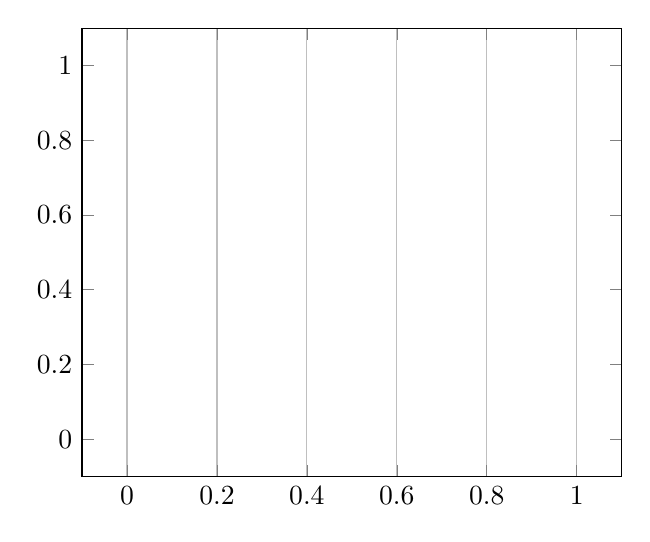
\begin{tikzpicture}
	\begin{axis}[xmajorgrids]
	\smallplotstest
	\end{axis}
\end{tikzpicture}

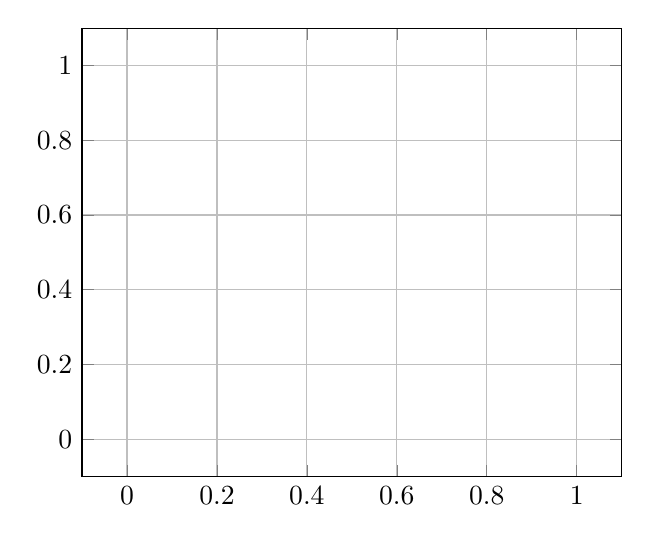
\begin{tikzpicture}
	\begin{axis}[ymajorgrids,xmajorgrids]
	\smallplotstest
	\end{axis}
\end{tikzpicture}

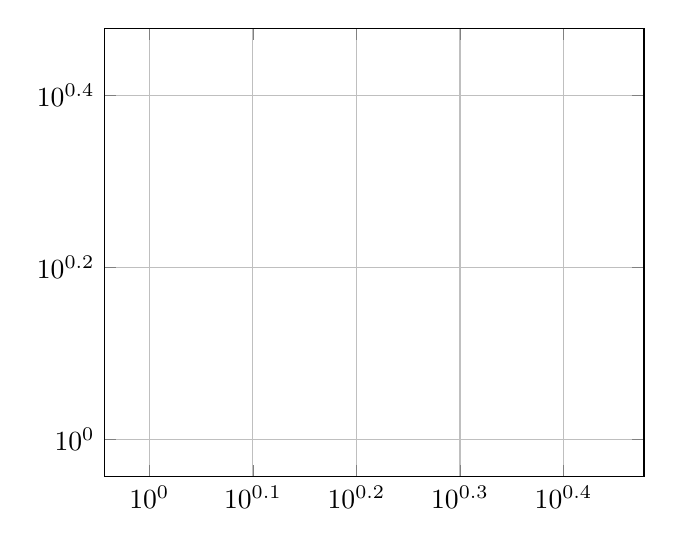
\begin{tikzpicture}
	\begin{loglogaxis}[ymajorgrids,xmajorgrids]
	\loglogtestplot
	\end{loglogaxis}
\end{tikzpicture}

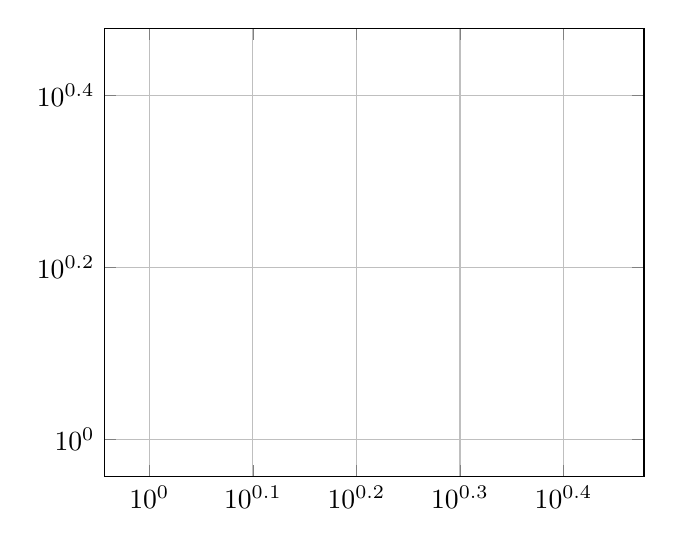
\begin{tikzpicture}
	\begin{loglogaxis}[grid=both]
	\loglogtestplot
	\end{loglogaxis}
\end{tikzpicture}

{
\pgfplotsset{every major tick/.append style={color=black,thick}}
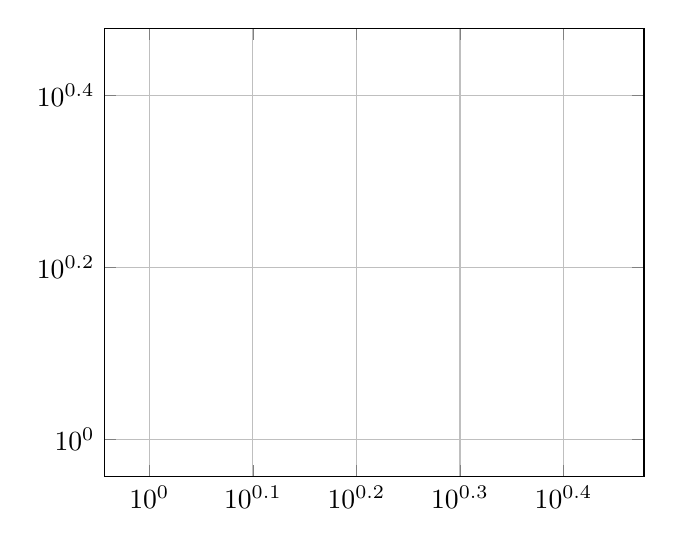
\begin{tikzpicture}
	\begin{loglogaxis}[grid=major]
	\loglogtestplot
	\end{loglogaxis}
\end{tikzpicture}

\pgfplotsset{every minor tick/.append style={color=black,thick}}
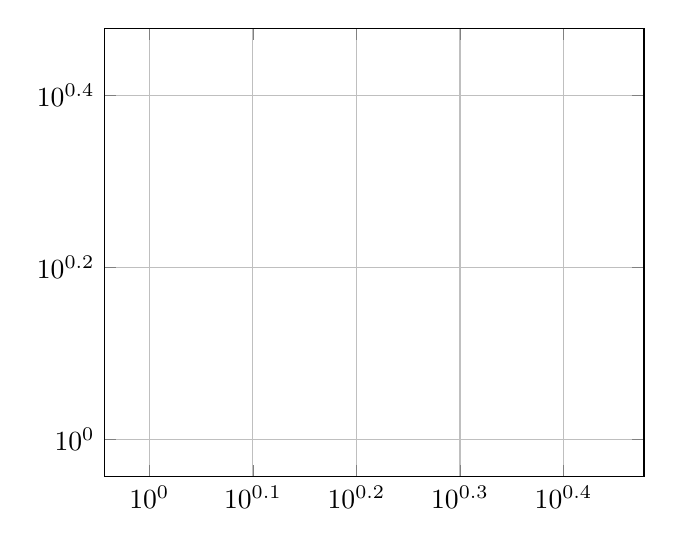
\begin{tikzpicture}
	\begin{loglogaxis}[grid=both]
	\loglogtestplot
	\end{loglogaxis}
\end{tikzpicture}
}

{
\pgfplotsset{grid=major}
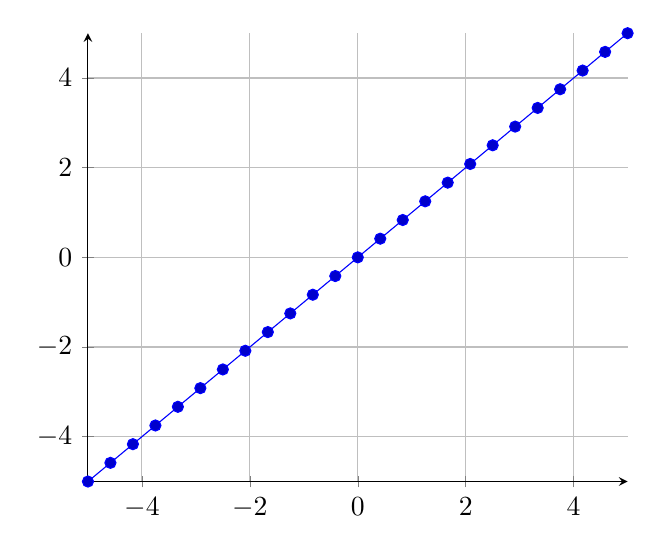
\begin{tikzpicture}
	\begin{axis}[axis x line=left,axis y line=left,grid=major]
		\addplot {x};
	\end{axis}
\end{tikzpicture}

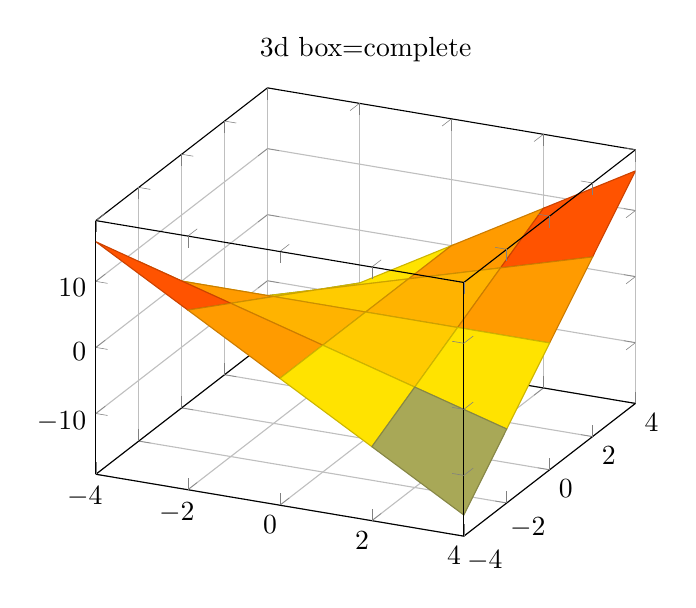
\begin{tikzpicture}
    \begin{axis}[
        3d box=complete,
        grid=major,
        title={3d box=complete},
        samples=5, domain=-4:4,
        xtick=data, ytick=data,
    ]
        \addplot3[surf] {x*y};
    \end{axis}
\end{tikzpicture}%

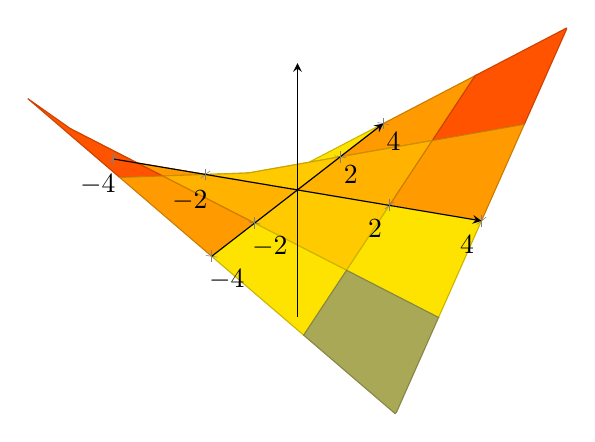
\begin{tikzpicture}
    \begin{axis}[
        axis lines=center,
        axis on top,
        samples=5, domain=-4:4,
        xtick=data, ytick=data,
        ztick=\empty, % no z ticks here
    ]
        \addplot3[surf] {x*y};
    \end{axis}
\end{tikzpicture}

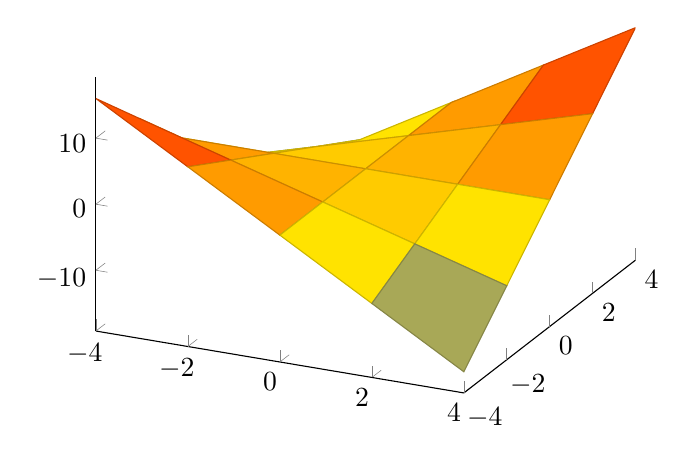
\begin{tikzpicture}
    \begin{axis}[
        axis lines*=left,
        samples=5, domain=-4:4,
        xtick=data, ytick=data,
    ]
        \addplot3[surf] {x*y};
    \end{axis}
\end{tikzpicture}

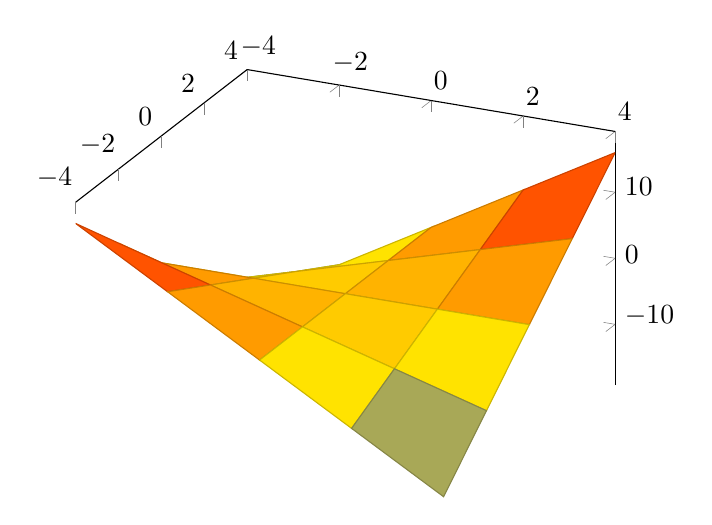
\begin{tikzpicture}
    \begin{axis}[
        axis lines*=right,
        samples=5, domain=-4:4,
        xtick=data, ytick=data,
    ]
        \addplot3[surf] {x*y};
    \end{axis}
\end{tikzpicture}

}

\testsection{Tick lines test}
\testsubsection{xmajorticks=false,xminorticks=true}
\begin{tikzpicture}
	\begin{loglogaxis}[xmajorticks=false,xminorticks=true]
	\loglogtestplot
	\end{loglogaxis}
\end{tikzpicture}

\testsubsection{ymajorticks=false,yminorticks=false}
\begin{tikzpicture}
	\begin{loglogaxis}[ymajorticks=false,yminorticks=false]
	\loglogtestplot
	\end{loglogaxis}
\end{tikzpicture}

\testsubsection{ticks=none}
\begin{tikzpicture}
	\begin{loglogaxis}[ticks=none]
	\loglogtestplot
	\end{loglogaxis}
\end{tikzpicture}

\testsubsection{ticks=major}
\begin{tikzpicture}
	\begin{loglogaxis}[ticks=major]
	\loglogtestplot
	\end{loglogaxis}
\end{tikzpicture}

\testsection{TikZ-coordinate system ``axis''}
\begin{tikzpicture}
\begin{axis}
\smallplotstest
\axispath\draw (axis cs:0.5,0.6) -- (axis cs:-1,0);
\end{axis}
\end{tikzpicture}

\begin{tikzpicture}
	\begin{loglogaxis}
	\axispath\draw 
		(axis cs:18943,2.873391e-05) |- (axis cs:47103,8.437499e-06);
	\loglogtestplot
	\end{loglogaxis}
\end{tikzpicture}


\testsection{Grid styles and axis line styles}
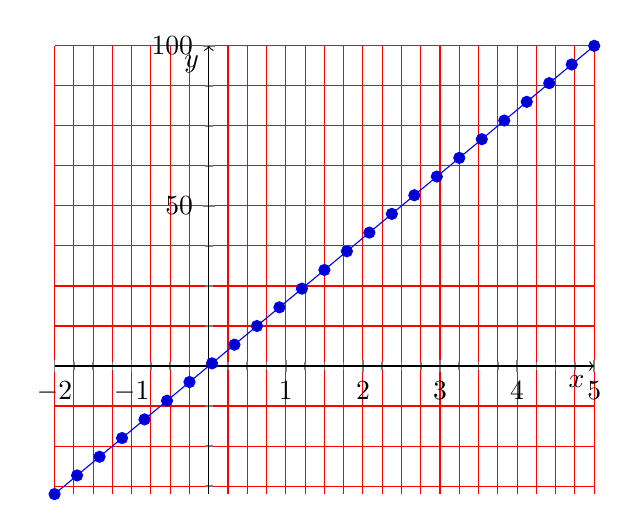
\begin{tikzpicture}
	\begin{axis}[
		axis x line=center,
		axis y line=center,
		 enlargelimits=false,
		grid=both,
		minor tick num=3,
		grid style={draw=red},
		tick style={semithick},
		tick align=center,
		xlabel=$x$,
		ylabel=$y$,
		every axis x label/.style={at={(current axis.right of origin)},anchor=north east},
		every axis y label/.style={at={(current axis.above origin)},anchor=north east},
		axis line style={->},
	]
	\addplot plot[domain=-2:5] (\x,20*\x);
	\end{axis}
\end{tikzpicture}
